\section{Case Studies}
\label{app:case_studies}

We provide case studies in this section, for both success and failed cases. Note: the 
\includegraphics[height=2em]{figures/loop.png} in every case figure means reuse the agent.
\subsection{Case 1 - Comparison Multi-hop QA}
\begin{figure}[ht!]
\centering

\includegraphics[width=0.5\linewidth]{figures/case1.png}
    \caption{Case 1 - Comparison Multi-hop QA}
    \label{fig:case1}
\end{figure}

Case 1 (Fig. \ref{fig:case1}) exemplifies an optimal Comparison Multi-hop reasoning pattern: the orchestrator produces a parallel topology to independent entity facts (each movie’s country) are retrieved in parallel, followed by a serial aggregation step for comparison. Such a parallel-then-serial decomposition improves efficiency, minimizes redundancy, and scales naturally to multiple entities, demonstrating functional differentiation between knowledge grounding and reasoning control. 
\subsection{Case 2 - Causal Multi-hop QA}
\begin{figure}[ht!]
\centering

\includegraphics[width=0.6\linewidth]{figures/case2.png}
    \caption{Case 2 - Causal Multi-hop QA}
    \label{fig:case2}
\end{figure}

For this causal multi-hop question (Fig. \ref{fig:case2}), \hero handles it by explicitly separating retrieval of causal evidence from reasoning over uncertainty. First, the system identifies the target entity (Jesus) and retrieves relevant historical and biblical sources describing the crucifixion and its contributing factors. Then, the reasoning module evaluates the retrieved evidence, accounting for ambiguity or contested interpretations, to determine whether the exact cause is definitively known. By maintaining this serial, dependency-aware workflow, \hero ensures that each reasoning hop builds on grounded evidence, minimizing hallucinations and producing a high-confidence answer. This functional differentiation between experience-grounded retrieval and adaptive causal reasoning allows HERA to robustly handle multi-hop questions where cause and certainty must be inferred sequentially.

\subsection{Case 3 - Temporal Multi-hop Q}
\begin{figure}[ht!]
\centering
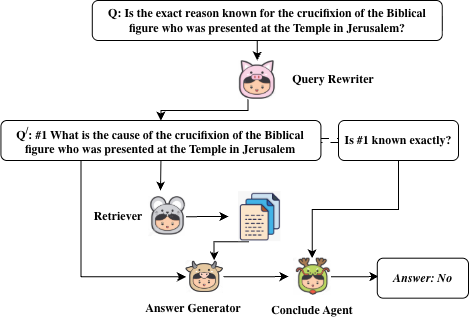
\includegraphics[width=0.5\linewidth]{figures/case3.png}
    \caption{Case 3 - Temporal Multi-hop QA}
    \label{fig:case3}
\end{figure}
Case 3 (Fig.\ref{fig:case3}) requires computing the temporal intersection of two activity periods, which demands not just parallel retrieval but a subsequent arithmetic-logical operation on the retrieved intervals. The system correctly decomposes the query and retrieves accurate individual activity periods: 1914–1938 for Hutchison and 1921–1944 for Howard. However, the Answer Generator returns ``1914–1944" — the union of the two intervals rather than their intersection (which would correctly be 1921–1938).
This failure reveals a fundamental limitation: the system lacks an explicit set-theoretic reasoning module. This suggests that for questions requiring numerical or logical operations over retrieved facts, a dedicated symbolic computation step is necessary. The failure is not a retrieval failure but a reasoning composition failure — a distinction with important implications for system design.

\subsection{Case 4 - Intersection Multi-hop QA}

\begin{figure}[ht!]
\centering
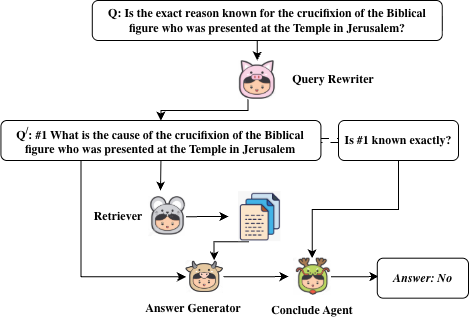
\includegraphics[width=0.5\linewidth]{figures/case4.png}
    \caption{Case 4 - Intersection Multi-hop QA}
    \label{fig:case4}
\end{figure}
For Case 4 (Fig.\ref{fig:case4}), which is a Intersection Multi-Hop type, the error illustrates a critical challenge in handling multi-entity property overlap. The pipeline’s goal is to identify a property that applies to both Pavel Alexandrov and Valentin Turchin. Here, the intended property is ``Soviet". However, the Query Rewriter reformulated the query around ``what they were known for," shifting focus to professional achievements (mathematician, computer scientist) rather than shared nationality or affiliation. Consequently, the Retriever retrieved evidence on their careers, and the Evidence Selector highlighted disciplinary roles, leading the Conclude Agent to output ``scientists."

Insights from this case:
\begin{itemize}
    \item Intersection multi-hop questions require careful alignment of the property type, for example nationality, affiliation, or field must be explicitly targeted; otherwise, retrieval can be biased toward more salient but irrelevant attributes.
    \item Parallel entity retrieval is insufficient if the property semantics are ambiguous, as each agent may return correct facts individually, but the intersection reasoning fails if the property dimension differs.
    \item Conclude Agent reasoning is sensitive to initial decomposition: even small shifts in question framing (profession vs. nationality) propagate to a semantically plausible but incorrect intersection.
\end{itemize}
